\chapter{Einleitung}

\begin{fquote}[Mark Zuckerberg][Facebook CEO][2014]
Virtual reality was once the dream of science fiction. But the internet was also once a dream, and so were computers and smartphones. The future is coming.
\end{fquote}

\begin{fquote}[Tim Cook][Apple CEO][2017]
I think AR is [...] big, it’s huge. I get excited because of the things that could be done that could improve a lot of lives.
\end{fquote}

\section{Einführung}
Viele der einflussreichsten Technologieunternehmen arbeiten an der \emph{Virtual} bzw.\ \emph{Augmented Reality (VR} bzw.\ \emph{AR)}. Tim Cook ist überzeugt davon, dass die AR die nächste \emph{``big idea''} nach dem Smartphone wird \cite{theindependent2017apple}.

Nicht nur Großkonzerne wie Apple, Facebook oder Samsung arbeiten intensiv in diesem Bereich. Ein Start-up-Unternehmen namens \emph{Magic Leap} entwickelt eine AR Brille und wird von Investoren in Billionenhöhe unterstützt \cite{kelly2016untold}. Laut einem Cover-Artikel der Zeitschrift \emph{Wire} ist die noch unter Verschluss gehaltene Technologie den Konkurrenzprodukten allen voraus. Das Release der Hardware ist Stand heute noch nicht bekannt, aber es lässt sich ein Trend erkennen, der die nächsten Jahre viele neue Möglichkeiten eröffnen wird und möglicherweise die Digitalisierung revolutionieren könnte.
Diese Arbeit wird sich mit einer Anwendung für die AR beschäftigen -- der Softwarevisualisierung. Die Spezialisierung auf AR kann nach der Abgrenzung von AR und VR besser nachvollzogen werden.

\paragraph{VR} ist eine Umgebung, in der der Betrachter vollkommen von einer computergenerierten Welt umgeben ist, die oft die reale Welt imitiert, aber auch rein fiktiv sein kann \cite{milgram1995augmented}.\\

Obwohl der Begriff AR zunehmend in der Industrie Verwendung findet, entbehrt er doch einer einheitlichen Definition. In \cite{azuma1997survey} wird AR als \emph{"`Variation"'} von VR betrachtet. Dagegen vermittelt Milgrim in \cite{milgram1995augmented} ein vollständigeres Verständnis, weshalb sich die Begrifflichkeiten in dieser Arbeit daran anlehnen sollen. Nach Milgrim existieren die beiden entgegengesetzten Extreme der Realität und der Virtualität. Alles dazwischen ist die sogenannte \emph{Mixed Reality (MR)}.

\paragraph{MR} ist eine Umgebung, in der Elemente der realen und einer virtuellen Welt zusammen dargestellt werden \cite{kato1999marker}.\\

\begin{figure}[htb]
  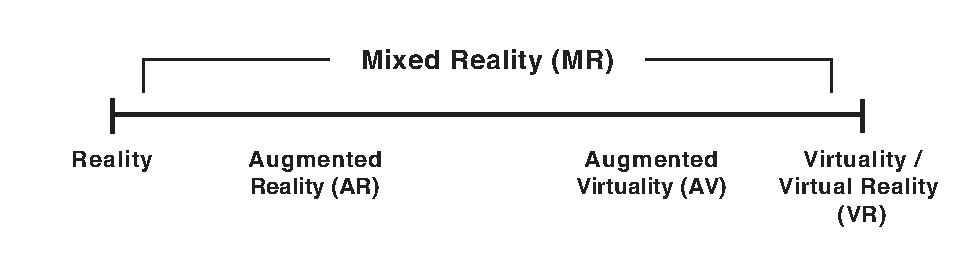
\includegraphics[width=.8\textwidth]{\figdir/rv-continuum}
  \caption{Abgewandelte Darstellung des Reality-Virtuality-Kontinuums aus \cite{milgram1995augmented}}
  \label{fig:rv-continuum}
\end{figure}

Dieses \emph{Reality-Virtuality-Kontinuum} ist in Abbildung \ref{fig:rv-continuum} dargestellt, in dem gut zu erkennen ist, dass AR zu der Mixed Reality gehört. In den meisten Quellen wie \cite{azuma1997survey, azuma2001recent, kato1999marker} wird bei der AR noch die Komponente der Interaktion aufgeführt. AR kann deshalb folgendermaßen definiert werden:

\begin{defbox}{AR}{ar}
   AR ist die Erweiterung der realen Welt durch computergenerierte Elemente, mit denen der Betrachter in Echtzeit interagieren kann.
\end{defbox}

Auch die \emph{Augmented Virtuality}, also die Erweiterung der virtuellen Welt durch reale Elemente, gehört zur MR.

Wie viele der einflussreichsten Menschen der Technologie-Industrie, sieht Tim Cook  mehr Zukunft in der AR, da, wie er in einem Interview sagt, diese Technologie nicht wie die VR die wirkliche Welt ausschließt, sondern die Realität erweitert und Teil von zwischenmenschlicher Kommunikation sein kann \cite{theindependent2017apple}.

Wir stellen uns ein Hologramm vor, dass auf einem Konferenztisch Gestalt annimmt und ein Software-System repräsentiert. Entwickler, Projektleiter oder auch Kunden versammeln sich um den Tisch und können miteinander interaktiv die Software betrachten, evaluieren und wichtige Informationen daraus ziehen.

Dies wäre mit VR nicht möglich, da der Betrachter von der Außenwelt abgeschottet ist. Deshalb wird im Zuge dieser Arbeit mit der Stand heut am weitesten ausgereiften Technologie der AR gearbeitet -- der \emph{HoloLens} von Microsoft.

\section{Motivation dieser Arbeit}
Die Technologie der AR bietet uns viele neue Möglichkeiten. Eine Motivation dieser Arbeit ist es sich produktiv mit einer neuen, zukunftsträchtigen Technologie zu beschäftigen. Das ist jedoch nur die eine Seite. Die weitaus größere Motivation ist, die zuvor noch nicht dagewesene Zugänglichkeit und Interaktion mit dreidimensionaler \emph{Visualisierung} auszunutzen. Visualisierung im Allgemeinen begegnet uns in vielen Bereichen unseres Lebens und nimmt eine wichtige Rolle ein.

Niemand konnte bislang unser Sonnensystem von außen betrachten. Dennoch haben wir alle eine ziemlich gute Vorstellung wie dieses aufgebaut ist. Durch die Visualisierung der Planeten und der Sonne entsteht in uns ein geistiges Abbild der Realität. Das Konzept komplexe Realitäten zu abstrahieren und zu visualisieren, um dadurch die Realität besser verstehen zu können, ist in vielen Disziplinen der Wissenschaft vertreten.

Neben Wissenschaften wie Physik, Chemie oder Biologie, nimmt Visualisierung
auch besonders in der Informatik eine wichtige Rolle ein. In vielen Bereichen müssen Informationen in eine visuelle Form gebracht werden, die für das menschliche Auge besser zu lesen sind.

Gerade bei komplexen Software-Systemen ist das der Fall. Soll zum Beispiel die zu Grunde liegende Struktur einer Software Außenstehenden erklärt werden, gelingt das mit einem visuellen Modell wie einem UML-Diagramm sicherlich besser, als nur in den Source-Code zu schauen.

So wie UML-Diagramme, war die Darstellungsform der Softwarevisualisierung bislang meist zweidimensional. Mit AR wird dieser Disziplin der Visualisierung jedoch wortwörtlich ein neuer Raum an Möglichkeiten eröffnet und in diese Arbeit soll diesen Raum ausfüllen.

\section{Zielsetzung}
Für die Zielsetzung einer 3D Softwarevisualisierung in der AR sollten zunächst die allgemeinen Ziele einer Softwarevisualisierung betrachtet werden. Softwarevisualisierung ist für Diehl die "`visualization of artifacts related to software and its development process"' \cite{diehl2007software}. Wird der Fokus mehr auf die Ziele, d.h. den Nutzen für den Betrachter gelegt, lässt sich Softwarevisualisierung wie folgt definieren:

\begin{defbox}{Softwarevisualisierung}{software-visualization}
Softwarevisualisierung ist die bildliche oder auch metaphorische Darstellung einer Software, um dem Betrachter durch Vereinfachung und Abstraktion das bessere Verständnis oder die einfachere Analyse von Software zu ermöglichen.
\end{defbox}

In dieser Arbeit soll das neue Konzept \emph{CodeLeaves} für eine solche Softwarevisualisierung in der AR vorgestellt und im Detail ausgearbeitet werden.

Dabei soll CodeLeaves, im Vergleich zu andern 3D Softwarevisualisierungen, die Vorteile der Dreidimensionalität optimal ausnutzen.

Im Vorfeld dieser Arbeit wurden in einer Studie Metriken gesammelt, die eine gute Softwarevisualisierung bzw. CodeLeaves unterstützen sollte.

Es sollen dynamische und statische Metriken zur Erkennung von Anomalien in einer Software unterstützt werden. Ebenfalls soll die Darstellung der Struktur und der darauf abgebildeten Abhängigkeiten innerhalb einer Software möglich sein.

Durch weitere Expertengespräche sollen Userstories erstellt werden um den Mehrwert des neuen Konzepts validieren zu können.

Um diesen Anforderungen gerecht zu werden, soll für CodeLeaves ein sprachunabhängiges Datenmodell entworfen werden, dass alle geforderten Metriken unterstützt.

Der Praktische Teil dieser Arbeit soll die prototypische Entwicklung von CodeLeaves für die HoloLens sein.

\section{Aufbau der Arbeit}
Im Kapitel \ref{ch:concept} wird das Konzept von CodeLeaves vorgestellt. Dabei wird zunächst unter Betrachtung alternativer Ansätzen begründet, wieso ein neues Konzept sinnvoll ist, um dann in Abschnitt \ref{sec:idea} genauer auf das Konzept einzugehen. Die Befragung von Experten der Softwareanalyse und die daraus abgeleiteten Anforderungen an CodeLeaves in Abschnitt \ref{sec:requirements} schließen das erste Kapitel ab.

Das Kapitel \ref{ch:data-model} beschäftigt sich mit der Entwicklung eines geeigneten Datenmodells für CodeLeaves. Es werden vorhandene Datenmodelle auf Tauglichkeit für CodeLeaves überprüft und Rücksprache mit erfahrenen Software-Ingenieuren gehalten.

Aufbauend auf das entwickelte Datenmodell, wird das Konzept von CodeLeaves in Kapitel \ref{ch:modelling} theoretisch weiter ausgearbeitet. Darunter fällt die Positionierung der Bäume auf einer Grundfläche und die Länge, Dicke und der Winkel der einzelnen Äste. Parallel zur Theorie wird aufgezeigt, wie sich CodeLeaves in Unity für die HoloLens modellieren lässt.

Die Interaktion mit CodeLeaves soll Thema des Kapitel \ref{ch:interaction} sein. Besonders die Abhängigkeiten von Artefakten einer Software sollen mithilfe von CodeLeaves interaktiv exploriert werden können.

Das Kapitel \ref{ch:conclusion} fasst die Ergebnisse der Arbeit zusammen und ein Ausblick auf zukünftige Verwendung und weiterführende Arbeiten runden die Arbeit ab.

\chapter{Das Konzept CodeLeaves}
\label{ch:concept}

\section{CodeLeaves und die Metapher Software-Wald}
\label{sec:idea}

\emph{``Hierarchies are almost ubiquitous [...]''} \cite{robertson1991cone} halten Robertson \emph{et al.}
 schon 1991 bei der Visualisierung von hierarchischen Informationen fest. So auch bei der Struktur einer Software. Jede Software mit einer geschachtelten Paketstruktur ist hierarchisch und kann in einer Baumstruktur dargestellt werden. \emph{"`Bäume sind eine der wichtigsten Datenstrukturen, die besonders im Zusammenhang mit hierarchischen Abhängigkeiten und Beziehungen zwischen Daten von Vorteil sind."'} \cite{ernst2016grundkurs} stellen auch Ernst \emph{et al.} fest. Draus folgt, dass die Darstellung von Software als Baum oder auch Bäume sinnvoll ist.

Der Baum in der Informatik zeugt von einer ursprünglichen Metapher -- der Baum, wie er draußen in der Natur wächst. Da dieser unbestritten dreidimensional ist, liegt eine Softwarevisualisierung für die Dreidimensionalität mit einer realitätsnäheren Interpretation der Baum-Metapher nahe. Werden die Bäume, die im zweidimensionalen meist von oben nach unten gezeichnet wird, in 3D in natürlicher Wuchsrichtung modelliert und mehrere Bäume für eine Software verwendet, entsteht eine neue Metapher: der \emph{Software-Wald}.

CodeLeaves stellt ein Konzept dar, dass sich die Metapher des Software-Waldes zu nutze macht und wird im Folgenden auf High-Level-Ebene skizziert und danach genauer erläutert:

\begin{definitionbox}{\textbf{Konzept:} CodeLeaves}
  \begin{enumerate}
    \item Die Struktur der Software wird mit nach oben wachsenden Bäumen dargestellt.
    \item Jedes Paket im \emph{Root-Verzeichnis} wird als einzelner Baum auf einer Ebene -- dem \emph{Waldboden} -- dargestellt.
    \item Die Blätter der Bäume entsprechen den Softwareartefakten (z.B. Klassen) und können durch ihre Farbe eine beliebigen Metrik visualisieren. 
    \item Zwischen den Bäumen entsteht ein \emph{Wurzelgeflecht}, was die aggregierten Abhängigkeiten zwischen den Paketen darstellt.
    \item Abhängigkeiten oder Aufrufe zwischen einzelnen Softwareartefakten werden aggregiert über die Elternpakete als farbige bzw. Dicke der Äste dargestellt oder alternativ als direkte \emph{Spinnweben} zwischen den Bäumen.
  \end{enumerate}
\end{definitionbox}

\paragraph{Punkt 1} ist dafür verantwortlich, dass die Softwarevisualisierung nahe an der tatsächlichen Software ist, wie sie ein Entwickler in seiner Code-Base gewöhnt ist. Das heißt, diejenigen, die auch tatsächlich mit der Software arbeiten, finden sich aufgrund der bekannten Baumstruktur auch in der Visualisierung schnell zurecht, ohne jedes Softwareartefakt auszuwählen, um zu sehen, mit welchem sie es zu tun haben. Im Fachjargon wird hier von der \emph{Habitability} gesprochen, also wie schnell oder gut sich ein Betrachter in einer Software oder auch deren Visualisierung "`zuhause"' fühlt \cite{wettel2007program}.

\paragraph{Punkt 2} ist weitgehend selbsterklärend. Durch Darstellung der Software in mehreren Bäumen entsteht erst der Software-Wald und die Pakete im Root-Verzeichnis als Wurzeln der Bäume zu verwenden bietet sich an. Das schließt jedoch nicht aus, dass Unterpakete als neuer Waldboden verwendet wird. Interaktion mit dem Waldboden soll Teil des Kapitel \ref{ch:interaction} sein.

\paragraph{Punkt 3} bedeutet, dass in CodeLeaves durch die Farbe der Blätter ein \emph{Laubdach} entsteht, dass eine gute Übersicht über eine ausgewählte Metrik der Software gibt. Beispielsweise kann der Farbe der Blätter die Code-Coverage der einzelnen Softwareartefakte (siehe Definition \ref{def:softartefact}) zugewiesen werden. Mit einer Skala von Grün bis Rot kann dann der Software-Wald bei guter Testabdeckung im sommerlichen Grün erstrahlen, oder bei einer weniger guten Coverage eher in den Herbst übergehen. Die Färbung des Laubdachs ist flexibel auf jegliche Metrik anwendbar, die bei der betrachteten Software zur Verfügung steht.

\begin{defbox}{Softwareartefakt}{softartefact}
  Ein Softwareartefakt wird in dieser Arbeit als Überbegriff für die kleinste betrachtete Einheit der Software verstanden. Das können bei objektorientieren Sprachen typischerweise Klassen, aber auch bei feinerer Granularität einzelne Funktionen innerhalb einer Klasse sein. Auch die Betrachtung von Dateien, die mehrere Klassen enthalten können, sind denkbar.
\end{defbox}

\paragraph{Punkt 4} bietet einen goßen Vorteil gegenüber der Zweidimensionalität. In Abbildung \ref{fig:3d-advantage} wird rechts das Prinzip des Wurzelgeflechts mit einem minimalistischen Beispiel illustriert.

\begin{figure}[htb]
  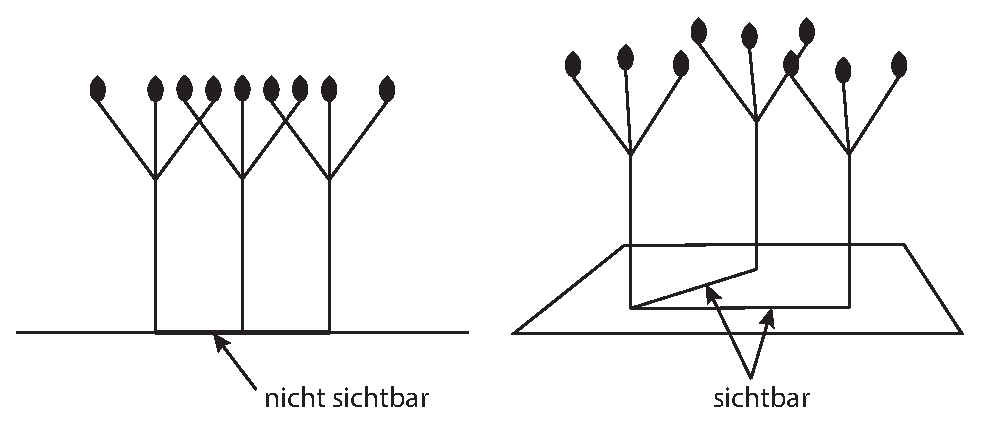
\includegraphics[width=.8\textwidth]{figures/3d-advantage}
  \caption{Vorteil der Dreidimensionalität bei der Darstellung von Abhängigkeiten}
  \label{fig:3d-advantage}
\end{figure}

Die Abhängigkeiten zwischen den Bäumen wird auf einen Blick ersichtlich. Betrachtet man die Bäume in 2D, wie es im linken Teil der Abbildung dargestellt ist, verschwinden die Abhängigkeiten hintereinander und sind nicht zuzuordnen.

\paragraph{Punkt 5} heißt, dass die Abhängigkeiten einer Software sehr übersichtlich auf die Struktur der Software abgebildet werden können, ohne diese zu beeinflussen. Für das besser Verständnis bedarf es einer Definition der Aggregation von Abhängigkeiten.

\begin{splitbox}{Aggregation von Abhängigkeiten}{aggregation}
Bei der Aggregation von Abhängigkeiten zwischen Softwareartefakten werden die Abhängigkeiten nicht direkt dargestellt, sondern über die Eltern-Pakete geleitet. Seien $x, y$ Pakete und Softwareartefakt $A \in x$ besitze eine Abhängigkeit zu Softwareartefakt $B \in y$, dann geht die Abhängigkeit von $A$ zu einem zusätzlich Konstrukt $\Psi_x$, das das Pakets $x$ repräsentiert. Angenommen $x$ und $y$ befinden sich zudem im Paket $z$, dann geht die aggregierte Abhängigkeit entweder direkt von $\Psi_x$ zu $\Psi_y$, oder weiter über $\Psi_z$ zu $\Psi_y$ und schließlich $B$.
\tcblower
%\raggedright
%Beispiel in CodeLeaves:\par\vspace{.6cm}
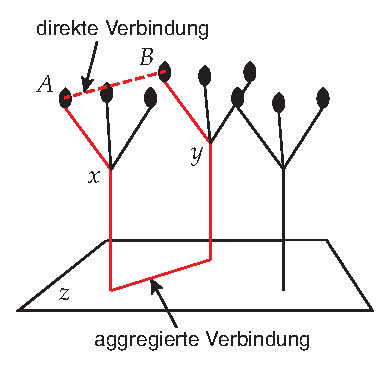
\includegraphics[width=\linewidth]{figures/aggregation}
\end{splitbox}

Auf der rechten Seite der Definition \ref{def:aggregation} ist eine aggregierte Abhängigkeit am Beispiel von CodeLeaves zu sehen. Die $\Psi$ in CodeLeaves sind die Knoten der Bäume, an denen die Äste zusammen laufen und im Spezialfall des Root-Verzeichnisses, der Waldboden.

Bei mehreren Abhängigkeiten zwischen Nachbar-Paketen, überlagern sich die aggregierten Abhängigkeiten zwangsläufig. Falls in unserem Beispiel eine weitere Abhängigkeit von Paket $x$ zu Paket $y$ bestünde, würden sich die Abhängigkeiten von $\Psi_x$ bis $\Psi_y$ überlagern. Daraus ergibt sich, dass nicht jede aggregierte Abhängigkeit ohne Interaktion zwangsläufig eindeutig zuzuordnen ist.

Wird aber bei jeder Kante, sei es ein Ast, Stamm, oder Wurzel, die Anzahl an überlagernden Abhängigkeiten als Dicke der Kante dargestellt, bekommt der Betrachter eine gute Übersicht über die Gesamtheit der Abhängigkeiten. Durch Interaktion mit einzelnen Kanten, oder sogar des ganzen Waldbodens, soll eine fein granulärere Analyse der Abhängigkeiten möglich sein.

Das zweite Element von Punkt 5 sind die Spinnweben. Damit lassen sich die Abhängigkeiten direkt darstellen. Um bei großen Software-Systemen aber die Übersicht über den Wald nicht zu verlieren, sollten diese mithilfe der Interaktion des Nutzers flexibel aktivierbar sein.

\section{Vergleich mit anderen Konzepten}
\label{sec:comparison}

Im Vorfeld dieser Arbeit wurde in \cite{puetz2017softwarevisualisierung} evaluiert, was eine gute Softwarevisualisierung ausmacht und unterstützen sollte. Ausgehend davon, wurden vorhandene 3D Visualisierungen und andere mögliche Konzepte miteinander verglichen. Die Ergebnisse dieser Untersuchung, soll in Folgenden vorgestellt werden.

Um herauszufinden welchen Mehrwert sich Nutzer einer Softwarevisualisierung von dieser versprechen, wurde eine Umfrage in der QAware GbmH durchgeführt. Die QAware ist ein Projekthaus mit den Kerngeschäften Diagnose, Sanierung, Exploration und Realisierung von Software \cite{qaware2017it-probleme}. Durch die Erfahrung in Projekten für namhafte Kunden, zeichnen sich die Mitarbeiter durch fundiertes Wissen und Expertise aus. Es wurden insgesamt 22 Mitarbeiter mit unterschiedlichen Rollen in der Softwareentwicklung befragt.

\begin{figure}[hbt]
\begin{tikzpicture}
  \begin{axis} [
    width = \textwidth,
    height = 8cm,
    symbolic x coords={Lines of Code, Komplexität, Coverage, Struktur, Abhängigkeiten, Code-Violations, Anzahl Aufrufe, Ausführungszeiten, Laufzeitfehler, Ressourcen-Auslastung, Evolution der Statik, Evolution eins Themas},
    xtick={Lines of Code, Komplexität, Coverage, Struktur, Abhängigkeiten, Code-Violations, Anzahl Aufrufe, Ausführungszeiten, Laufzeitfehler, Ressourcen-Auslastung, Evolution der Statik, Evolution eins Themas},
    x tick label style={rotate=45, anchor=east, align=center},
    major x tick style = transparent,
    axis lines = left,
    axis line style = {-},
    ymajorgrids = true,
    ylabel=Anzahl,
    legend style = {at={(.99,.98)}, anchor=north east, legend columns=-1, column sep=1ex},
    ymin=0,
    bar width=5mm,
    ybar=-0.5cm,
    enlarge x limits={abs=0.6cm}
  ]
    \addplot[style={fill=primary}]
      coordinates {(Lines of Code, 1) (Komplexität, 3) (Coverage, 1) (Struktur, 5) (Abhängigkeiten, 7) (Code-Violations, 4)};
    \addplot[style={fill=secondary}]
      coordinates {(Anzahl Aufrufe, 5) (Ausführungszeiten, 5) (Laufzeitfehler, 1) (Ressourcen-Auslastung, 1)};
    \addplot[style={fill=tertiary}]
      coordinates {(Evolution der Statik, 3) (Evolution eins Themas, 1)};

    \legend{Statik, Dynamik, Evolution}

  \end{axis}
\end{tikzpicture}
\caption{Von Mitarbeitern der QAware gewünschte Informationen} \label{fig:survey}
\end{figure}

In Abbildung \ref{fig:survey} ist zu sehen, wie oft welche Metriken genannt wurden. Alle Metriken lassen sich in die drei Kategorien der Softwarevisualisierung aus \cite{diehl2007software} einordnen und sind farbig entsprechend gruppiert.

\paragraph{Statik} sind die Informationen, die ohne die Ausführung der Software generiert werden können \cite{diehl2007software}. Darunter fallen die Metriken, die als Zahl zu jedem Softwareartefakt zugeordnet werden können und damit zueinander in Relation gesetzt werden können. Genannt wurden LOC, Komplexität, Coverage und Code-Violations. Letzteres sind beispielsweise Verletzungen von vereinbarten \emph{Code-Conventions}. Die Informationen, die komplizierter zu visualisieren sind, stellen die Struktur und die Abhängigkeiten dar. Aus Abbildung \ref{fig:survey} geht hervor, dass diese Informationen gleichzeitig am meisten von Interesse sind.

\paragraph{Dynamik} beschreibt die Informationen, die zur Laufzeit einer Software generiert werden können \cite{diehl2007software}. Besonders oft wurden Ausführungszeiten von Softwareartefakten und Anzahl von Aufrufen genannt. Damit sind beispielsweise \emph{Bottlenecks} identifizierbar. Auch die Darstellung der Laufzeitfehler einer fehlerhaften Software sind für deren Analyse wichtig. Die Resourcen-Auslastung ist dabei auch hilfreich, wirkt sich jedoch wenig auf das 3D Modell der Softwarevisualisierung aus, da diese Informationen parallel zur eigentlichen Software existieren.

\paragraph{Evolution} beschreibt den zeitlichen Verlauf einer Software und stellt den Entwicklungsprozess in den Vordergrund \cite{diehl2007software}. Beispielsweise kann die Entwicklung statischer Metriken verfolgt werden. Mit der Evolution eines Themas ist gemeint, dass anhand die Entwicklung eines bestimmten Themas nachverfolgt werden kann.\\

Aus den von den Mitarbeiten gewünschten Informationen und weitern Rahmenbedingungen wurde in \cite{puetz2017softwarevisualisierung} folgende Kriterien aufgestellt, anhand derer vier verschiedene Modelle der 3D Softwarevisualisierung bewertet wurden.

\begin{itemize}
  \itemsep0pt
  \item Statische Metriken (z.B. Komplexität)
  \item Struktur
  \item Abhängigkeiten
  \item Dynamik (Primär Ausführungszeiten und Anzahl der Aufrufe)
  \item Evolution
  \item Habitability (vgl. Kapitel \ref{ch:concept} Punkt 1)
  \item Drilldown
  \item Technische Machbarkeit
\end{itemize}

Bei dem Kriterium Drilldown wurde bewertet, wie gut eine Visualisierung ihre Informationen von High-Level, bis hin zu Details darstellen kann.

Bei der technischen Machbarkeit wurde berücksichtigt, ob eine existierende Softwarevisualisierung für die HoloLens verwendbar ist. In Abbildung \ref{fig:alternatives} sind die untersuchten Alternativen abgebildet, darunter auch ein erster Entwurf von CodeLeaves.

\subsubsection*{CodeCity}
2007 stellten Wettel et al. CodeCity vor, die mithilfe der \textit{Stadt-Metapher} dreidimensionale Städte visualisiert, in denen Klassen als Gebäude und Pakete als Stadtviertel dargestellt werden \cite{wettel2007program, wettel2008visual, wettel2011software}. Für die Breite und Tiefe der Gebäude wurde für die Anzahl der Attribute (engl. \emph{number of attributes (NOA)}) und für die Höhe die Anzahl der Methoden (engl. \emph{number of methods (NOM)}) der visualisierten Klasse gewählt.

Die CodeCity ist als Konzept sehr durchdacht, bietet durch die Metapher gute Habitability und unterstützt die Darstellung der Evolution. Auch soll nach Wettel et al. die CodeCity die Analyse von Software im Vergleich zu herkömmlichen Analyse-Werkzeugen signifikant verbessern \cite{wettel2011software}.

Jedoch unterstützt CodeCity keine Dynamik und die Abhängigkeiten sind nur als direkte Verbindungen darstellbar, was bei größeren Software-Systemen sehr unübersichtlich wird. Die verfügbaren statischen Metriken sind begrenzt und vor allem ist die Technologie Stand heute nicht mehr produktiv einsetzbar \cite{puetz2017softwarevisualisierung}.

\newlength\fwidth
\setlength{\fwidth}{.49\textwidth}
\begin{figure}[htb]
  \centering
  \begin{subfigure}[b]{\fwidth}
   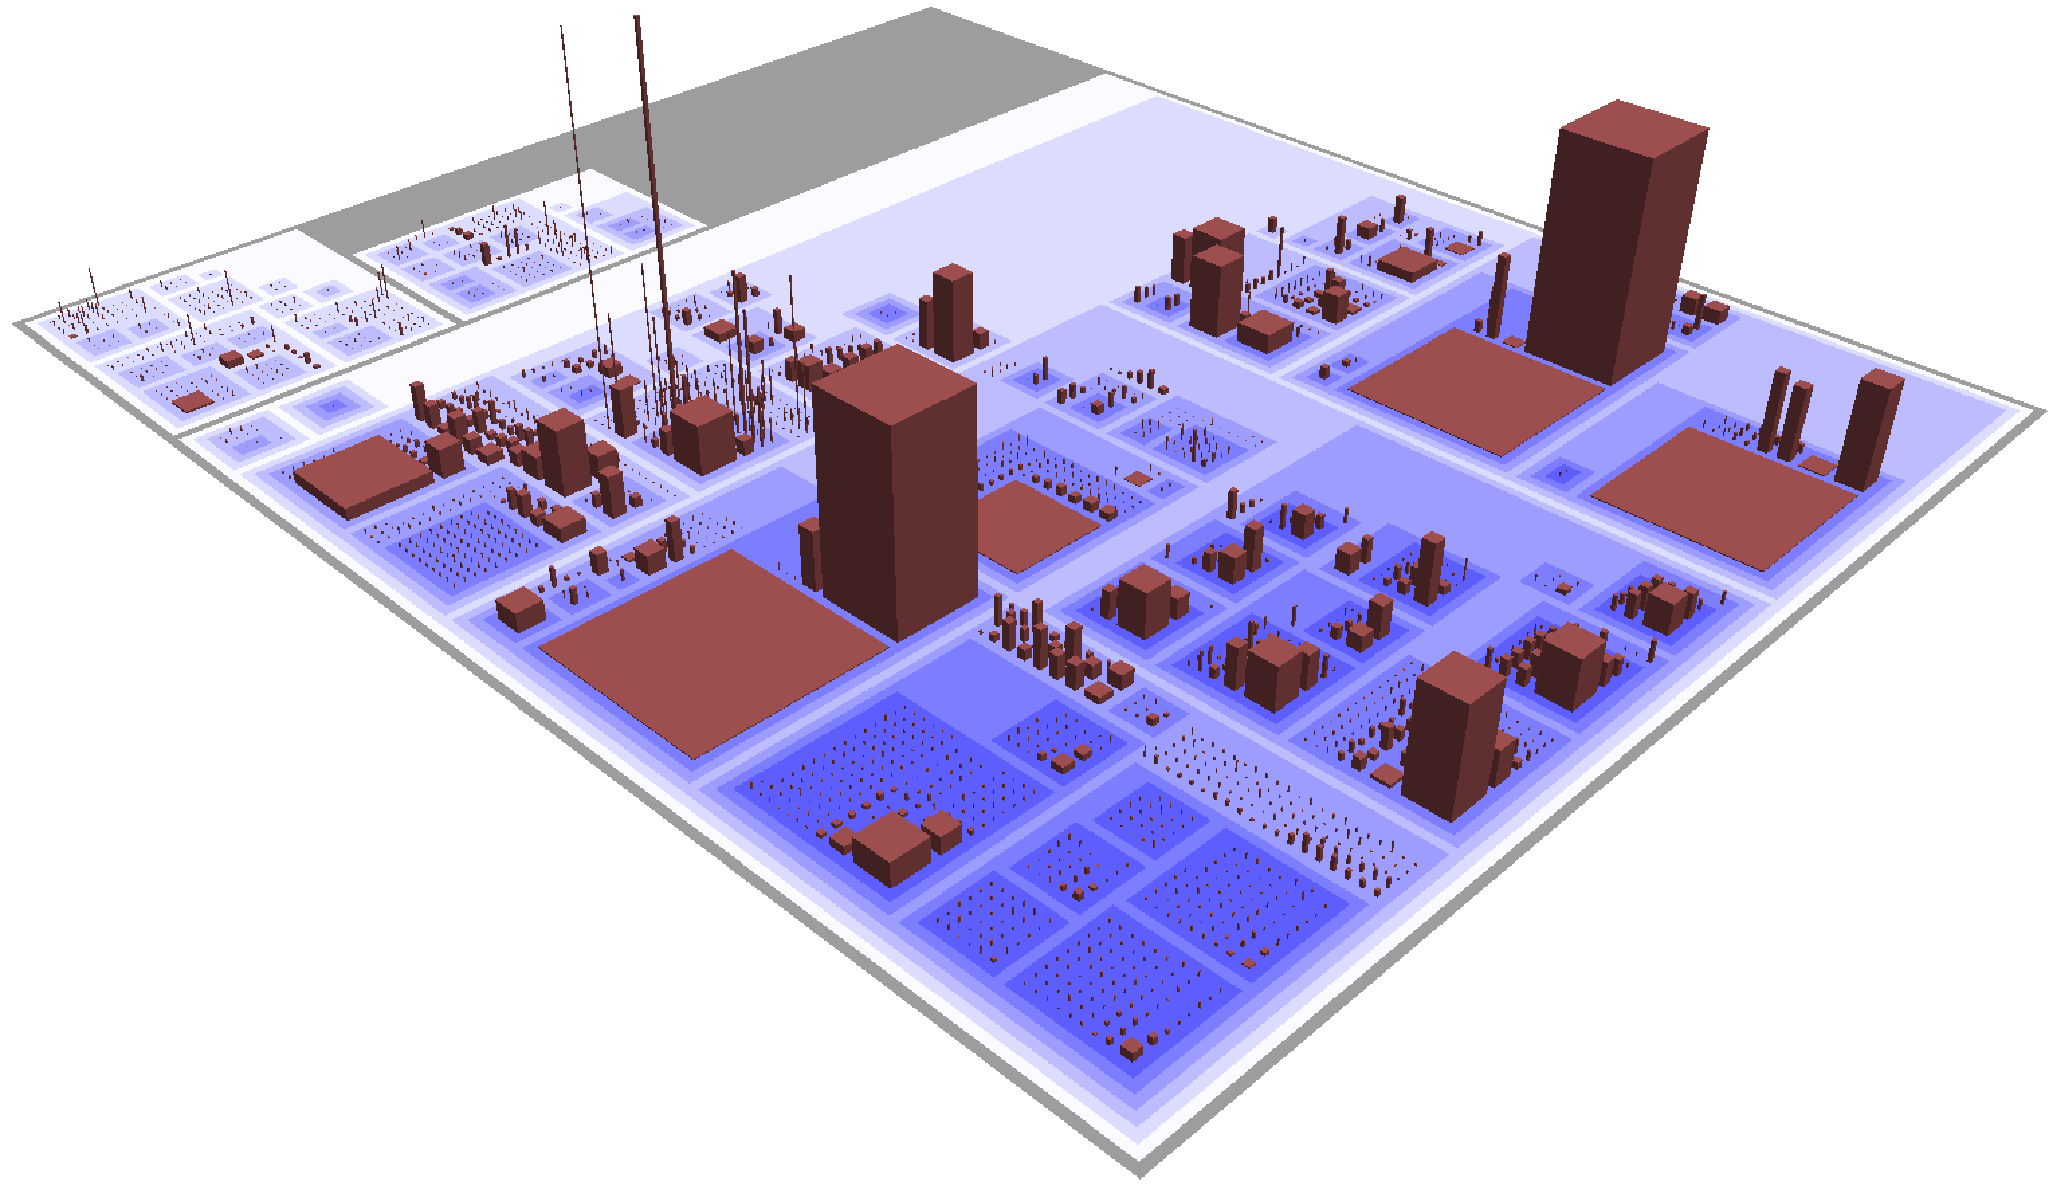
\includegraphics[width=\textwidth]{figures/code-city}
   \subcaption{CodeCity von ArgoUML \cite{wettel2008visual}} \label{fig:code-city}
  \end{subfigure}
  \hfill
  \begin{subfigure}[b]{\fwidth}
  	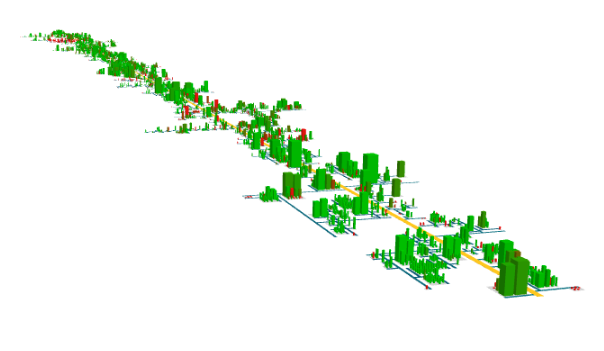
\includegraphics[width=\textwidth]{figures/softvis3d}
  	\subcaption{SoftVis3D mit Evostreet Layout} \label{fig:softvis3d}
  \end{subfigure}
  \hfill
  \vspace{1em}
  \begin{subfigure}[b]{\fwidth}
  	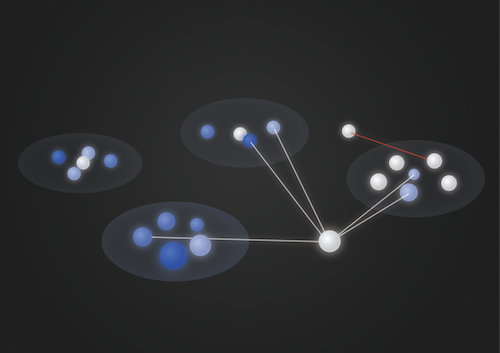
\includegraphics[width=\textwidth]{figures/code-universe}
  	\subcaption{Entwurf eines CodeUniverse} \label{fig:code-universe}
  \end{subfigure}
  \hfill
  \begin{subfigure}[b]{\fwidth}
  	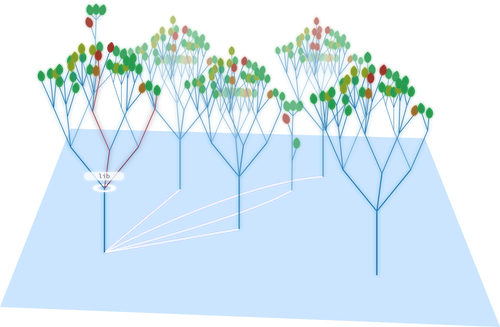
\includegraphics[width=\textwidth]{figures/code-leaves}
  	\subcaption{Erster Entwurf von CodeLeaves} \label{fig:code-leaves}
  \end{subfigure}
  \caption{CodeLeaves und alternative Modelle} \label{fig:alternatives}
\end{figure}

\subsubsection*{SoftVis3D}
SoftVis3D greift das Konzept der CodeCity auf und visualisiert als Plugin für SonarQube\footnote{SonarQube ist eine open-source Plattform für statische Code-Qualität, \url{https://www.sonarqube.org/}} Projekte direkt im Browser. Durch die direkte Anbindung an SonarQube, ist SoftVis3D hoch konfigurierbar und kann alle Metriken darstellen, die auch in SonarQube zur Verfügung. Neben dem \emph{District-Layout}, wie es in der CodeCity verwendet wird, unterstützt SoftVis3D darüber hinaus auch des \emph{Evostreet-Layout}, das ursprünglich in \cite{steinbruckner2013consistent} für die Evolution einer Software entworfen wurde. In diesem Layout, wie es in Abbildung \ref{fig:softvis3d} zu sehen ist, werden Pakete als Straßen dargestellt.

Die Evolution wird von SoftVis3D trotz Evostreet-Layout jedoch nicht unterstützt. Bei Die Abhängigkeiten wurde in früheren Versionen aggregiert dargestellt. Dafür wurden Pakete im Distrikt-Layout in übereinander liegenden Ebenen abgebildet und für $\Psi$ (vgl. Definition \ref{def:aggregation}) ein Hilfsgebäude benutzt, dass zu der darüberliegenden Ebene führt. Dadurch ging jedoch die Stadt-Metapher und die Übersichtlichkeit verloren. Die Dynamik kann in SoftVis3D ebenfalls nicht visualisiert werden. Die verwendete Technologie ist zwar mit \emph{WebGL} für den Browser State of the Art, aber für die HoloLens aktuell noch nicht sinnvoll einsetzbar \cite{puetz2017softwarevisualisierung}.

\subsubsection*{CodeUniverse}

Im Zuge der der Studie \cite{puetz2017softwarevisualisierung} wurde eine weitere Metapher evaluiert. Ähnlich wie in der Arbeit \cite{graham2004solar, balzer2004software}, wird die Software als Universum dargestellt. Die Softwareartefakte in Paketen gruppieren sich als Sterne in Galaxien. Statische Metriken können dann als Farbe und Größe der Sterne widergespiegelt werden. So können "`weiße Zwerge"' bis hin zu "`roten Riesen"' entstehen.

Das CodeUniverse ist für statische Metriken gut geeignet. Auch die Evolution ist mit der Entstehung von neuen Sternen und Galaxien gut vorstellbar. Die Struktur der Software ist zwar mit der Gruppierung der Sterne gegeben, aber weniger offensichtlich wie andere Konzepte. Bei der Visualisierung der Abhängigkeiten stößt das CodeUniverse aber an seine Grenzen. Durch direkte Verbindungen zwischen den Sternen lassen sich zwar Abhängigkeiten darstellen, aber bei großen Software-Systemen würde das schnell im Chaos enden. Auch in \cite{balzer2004software} wird beschrieben, dass eine übersichtliche Darstellung von Abhängigkeiten nur durch deren Aggregation erreicht werden kann. Deshalb wird in \cite{balzer2004software} ein Konzept entworfen, dass die Softwareartefakte mit einem \emph{"`hierarchischem Netz"'} verbindet. Dieses ist nichts anderes als die vorhandene Baumstruktur der Software und hat mit der Metapher des Universums auch nichts mehr zu tun. Folglich wären wir wieder bei dem neuen Konzept CodeLeaves angelangt.


\subsubsection*{Vorteile von CodeLeaves gegenüber anderen 3D Softwarevisualisierungen}
Die betrachteten Alternativen und weitere, haben gemein, dass sie zum einen Struktur, Dynamik und Evolution nicht vereinen. Zum anderen können Abhängigkeiten oder dynamische Aufrufe zwischen Softwareartefakten nicht ohne Verlust der Übersichtlichkeit angezeigt werden. CodeLeaves soll alle drei Kategorien der Softwarevisualisierung unterstützen und ist bei der Visualisierung der Struktur und der Abhängigkeiten den Alternativen überlegen. Durch die Baumstruktur, wie er auch in der Code-Base vorhanden ist, wird die Paket-Struktur eins zu eins wiedergegeben. Die aggregierten Abhängigkeiten lehnen sich an die Struktur an und beeinflussen diese nicht negativ. Durch das Wurzelgeflecht und die Spinnweben wird die Dreidimensionalität optimal ausgenutzt.

\section{Anforderungen an CodeLeaves}
\label{sec:requirements}

\chapter{Datenmodell}
\label{ch:data-model}
\section{FAMIX-Familie}

\chapter{Modellierung}
\label{ch:modelling}

\chapter{Interaktionskonzept}
\label{ch:interaction}
\chapter{Zusammenfassung und Ausblick}
\label{ch:conclusion}
		